\chapter{Usability Evaluation of Smart Cafeteria}
\label{chap:EvaluationSC}
In interactive system design, usability evaluation appears to be very vital
issue in the design life cycle and development process. Sometimes,
usability evaluation is performed in user-centric design at the very
beginning stage with low fidelity prototype such as paper based prototype; or at
requirements gathering stage using focus group and survey questionnaire to get
users' feedback which helps to find out more requirements to make a system
stable; and the modification process continues until the final version of the
product.


The usability evaluation goals of ``Smart Cafeteria" is to test usefulness of
the system, how easy the system to use, Satisfaction, learnability and find out
more requirements to improve the design. To know and figure out best evaluation
methods for ``Smart Cafeteria'', I have studied a couple of article, paper and
book which is discussed here.



\citet{Nielsen2003} define five usability components to assesses how easy user
interfaces are to use. These are Learnability, Efficiency, Memorability, Errors
and Satisfaction.

\citet{Dix2004} defines usability as quality attribute of a system that ensure
the efficiency, effectiveness and satisfaction of specified users to achieve
specified goals in particular environment. They suggested making a distinction
between evaluation by the users at early design stage using focus groups,
survey questionnaires and the evaluation by the designer or a usability expert
at completed system or functional prototype design stage as a cheap and quick
usability assessment. According to their consideration, there are four
approaches for expert analysis: cognitive walkthrough, heuristic evaluation, the
use of models and use of previous work.

In the cognitive walkthrough, the sequence of actions will be performed in order
to accomplish some known task by the users in the system and the principle focus
of the cognitive walkthrough methodology  is to establish how easy a system is
to learn.

Heuristic evaluation, developed by Jakob Nielsen and Rolf Molich, is performed
in design specification stage or early design evaluation stage but could also be
used on prototypes, fully functioning systems.

There are four approaches for user analysis too: empirical or experimental
methods, observational methods, query techniques, and methods that use
physiological monitoring.

Query techniques are a kind of evaluation techniques that is asking the user
about the interface directly and these could be useful in drawing out detail
about the user's view of a system and collect information about user
requirements and tasks. The main query techniques approaches are interview and
questionnaires.

Interviewing users with an interactive system about their experience is a direct
and structured way of collecting feedbacks and gathering information or
requirements.

Questionnaire is an alternative method of querying the user with different
question styles such as general opens ended, scalar, multiple choice and ranked
questions.


M. Ivory~\cite{Ivory2001} has shown in his thesis work that the activities that
may occur during the usability evaluation process.
\begin{enumerate}
\item Specify usability evaluation goals.
\item Determine UI aspects to evaluate.
\item Identify target users.
\item Select usability metrics.
\item Select evaluation method(s).
\item Select tasks.
\item Design experiments.
\item Capture usability data.
\item Analyze and interpret usability data.
\item Critique UI to suggest improvements.
\item Iterate the process if necessary.
\item Present results.
\end{enumerate}

\section{Evaluation Methodology}
From above definition and discussion of usability evaluation techniques, this
work has followed \textbf{user studies methodology and questionnaire} techniques
for evaluation. In the beginning of evaluation, the goal of evaluations are
defined; \textbf{(i) to test usefulness of the system, (ii) how easy the system
is to use, (iii) learnability and (iv) Satisfaction} to improve the design.


Then I have identified the \textbf{target users (students of University of
Trento)} for evaluation who are used to have lunch in cafeteria in the working
days. I have chosen ten (10) students; all of them takes lunch at cafeteria
more than three times in a week. In each session, I have discussed with them the
main goals and key features [section \ref{sec:keyFeaturesSC}] of the ``Smart
Cafeteria'' and given them some specific tasks to perform. The users had no
previous experience about the system and UI. The tasks were as follows:
\begin{itemize}
  \item \textbf{T1:} Perform Login.
  \item \textbf{T2:} Search Food Menu.
  \item \textbf{T3:} Create A Food Menu.
  \item \textbf{T4:} Search  Friends.
  \item \textbf{T5:} Check Your Diet Report.
  \item \textbf{T6:} Check Followers.
  \item \textbf{T7:} Check Time Schedule.
  \item \textbf{T8:} Check who are Following you.
  \item \textbf{T9:} Check friend's activities.
\end{itemize}

I have given to users simple tasks to perform, as I had mid-fidelity prototype
for both desktop and mobile application with the most important navigation
control and basic functionalities at that time. The reason for giving tasks was
because I wanted the users to browse the whole system at once and those tasks
would cover the present version of prototype. The task analysis and user
observation has done only for desktop prototype[subsection
\ref{subsec:UserObservation}].


After performing the tasks, I have presented some questionnaire to the users and
requested them to answer which covered the goal of usability evaluation of this
work. The questionnaire was built based upon the Likert scale and the users were
allowed to indicate their agreement or disagreement with a 7 point scale.

The usability evaluation has done for both desktop prototype[subsection
\ref{subsec:QuestionnaireDesktop}] and mobile prototype[subsection
\ref{subsec:QuestionnaireMobile}] followed by the same questionnaire.

\section{Evaluation Result}
\subsection{User Observation}
\label{subsec:UserObservation}
In the user observation phase, most of users were able to perform the task
correctly. There was one iteration conducted for testing the performance of the
users on using the user interfaces of Smart Cafeteria initially; but in future
there will be more iteration to conduct for making the system more usable. In
this phase, no bench mark time would be fixed, only observe users how many
attempts they need to perform the task. The scale of observation was from one
attempt to three attempts which indicate best case to worst case. There was also
a case unsuccessful which was meant user didn't find the option.

The outcome of the study of the user observation test for the tasks is presented
in details here.

%Perform Login and search Food menu
\begin{figure}[h!t]
\centering
\begin{subfigure}[b]{.5\textwidth}
  \centering
  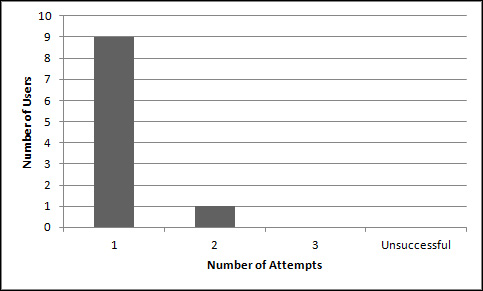
\includegraphics[width=0.9\textwidth]{ch5/Interview/EvaluationResult/PerformLogin.jpg}
\end{subfigure}%
\begin{subfigure}[b]{.5\textwidth}
  \centering
  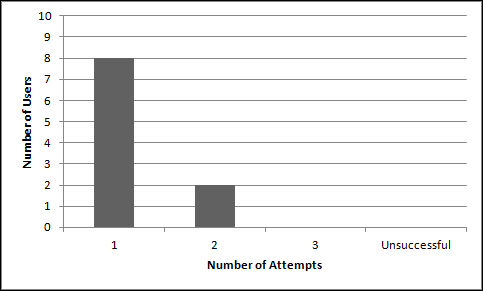
\includegraphics[width=0.9\linewidth]{ch5/Interview/EvaluationResult/SearchFoodMenu.jpg}
\end{subfigure}
\caption{Perform Login(Left).Search Food Menu(Right).}
\label{fig:EvaluationResult1}
\end{figure}

It is found that nine (9) users [figure \ref{fig:EvaluationResult1}] were able
to perform login in first attempt and only one (1) user needed two attempts. And
Eight (8) users were able to Search Food Menu in the first attempt without any
error and two (2) users took two attempts. In those tasks 100\% users are
successful.

%Create Food menu and Search friend
\begin{figure}[h!t]
\centering
\begin{subfigure}[b]{.5\textwidth}
  \centering
  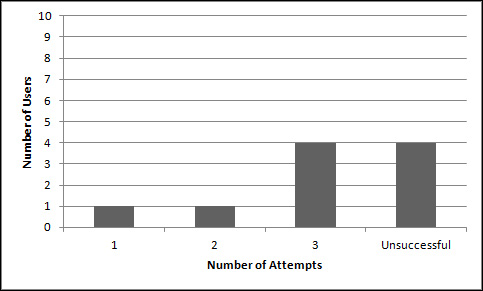
\includegraphics[width=0.9\textwidth]{ch5/Interview/EvaluationResult/CreateAFoodMenu.jpg}
\end{subfigure}%
\begin{subfigure}[b]{.5\textwidth}
  \centering
  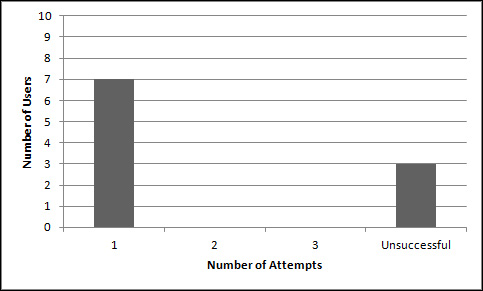
\includegraphics[width=0.9\linewidth]{ch5/Interview/EvaluationResult/SearchFriends.jpg}
\end{subfigure}
\caption{Create Food Menu(Left). Search friend(Right).}
\label{fig:EvaluationResult2}
\end{figure}

From the figure \ref{fig:EvaluationResult2}  we can see that 40\% of the users
were unsuccessfully in create food menu tasks and 30\% users were unable to
search their friends.


In the figure \ref{fig:EvaluationResult3}  shows that 60\% of the users were
able to perform these two tasks successfully in the first attempt and 100\% was
successful.
%Check your Diet Report and Check followers
\begin{figure}[h!t]
\centering
\begin{subfigure}[b]{.5\textwidth}
  \centering
  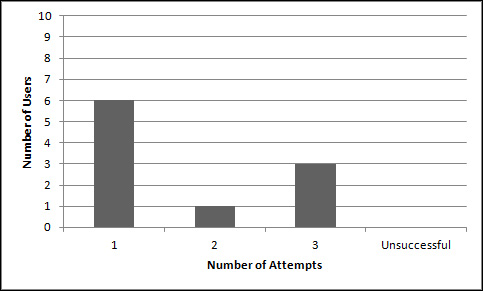
\includegraphics[width=0.9\textwidth]{ch5/Interview/EvaluationResult/CheckYourDietReport.jpg}
\end{subfigure}%
\begin{subfigure}[b]{.5\textwidth}
  \centering
  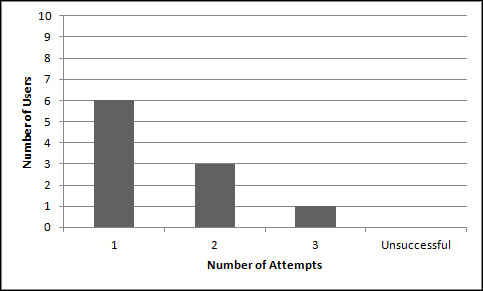
\includegraphics[width=0.9\linewidth]{ch5/Interview/EvaluationResult/CheckFollowers.jpg}
\end{subfigure}
\caption{Check your Diet Report(Left). Check followers(Right).}
\label{fig:EvaluationResult3}
\end{figure}

In case of checking time schedule [figure \ref{fig:EvaluationResult4}] and ``who
are following you'' [figure \ref{fig:EvaluationResult4}], 80\% and 70\% users
were able to perform the tasks successfully with only one attempt respectively.
%Check Time Schedule and Check who are Following you 
\begin{figure}[h!t]
\centering
\begin{subfigure}[b]{.5\textwidth}
  \centering
  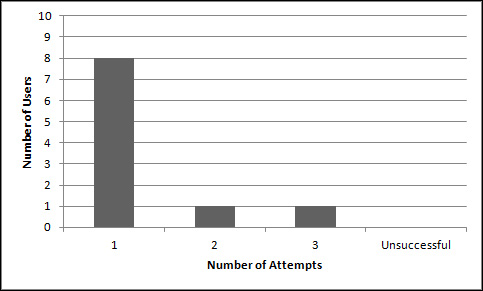
\includegraphics[width=0.9\textwidth]{ch5/Interview/EvaluationResult/CheckTimeSchedule.jpg}
\end{subfigure}%
\begin{subfigure}[b]{.5\textwidth}
  \centering
  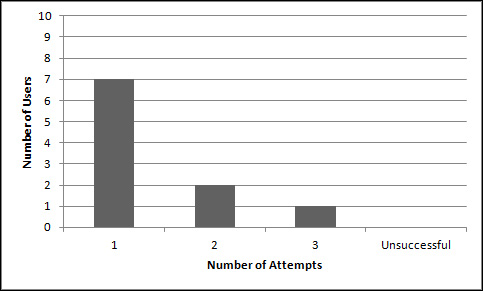
\includegraphics[width=0.9\linewidth]{ch5/Interview/EvaluationResult/CheckwhoareFollowingyou.jpg}
\end{subfigure}
\caption{Check Time Schedule(Left). Check who are Following you (Right).}
\label{fig:EvaluationResult4}
\end{figure}
\newpage
From the figure [\ref{fig:EvaluationResult5}] we can see that 90\% of the
users successfully done the task to check friend's activities successfully in
the first attempt.
%Check friend's activities
\begin{figure}[h!t]
\centering
\begin{subfigure}[b]{.5\textwidth}
  \centering
  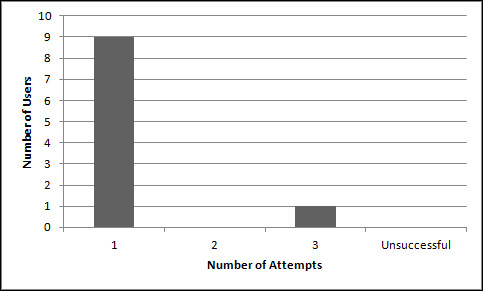
\includegraphics[width=0.9\textwidth]{ch5/Interview/EvaluationResult/CheckFriend'sActivities.jpg}
\end{subfigure}%

\caption{Check friend's activities}
\label{fig:EvaluationResult5}
\end{figure}
 
 In the figure [\ref{ComparisonofTasksPerformance}], we can see the
 comparison of the tasks performance of the users where create food menu and
 search friends only had 40\% and 30\% unsuccessful rate, otherwise the other
 task had satisfactory performance rate.

% Comparison�of�Task Performance
\begin{figure}[h!t]
    \centering
      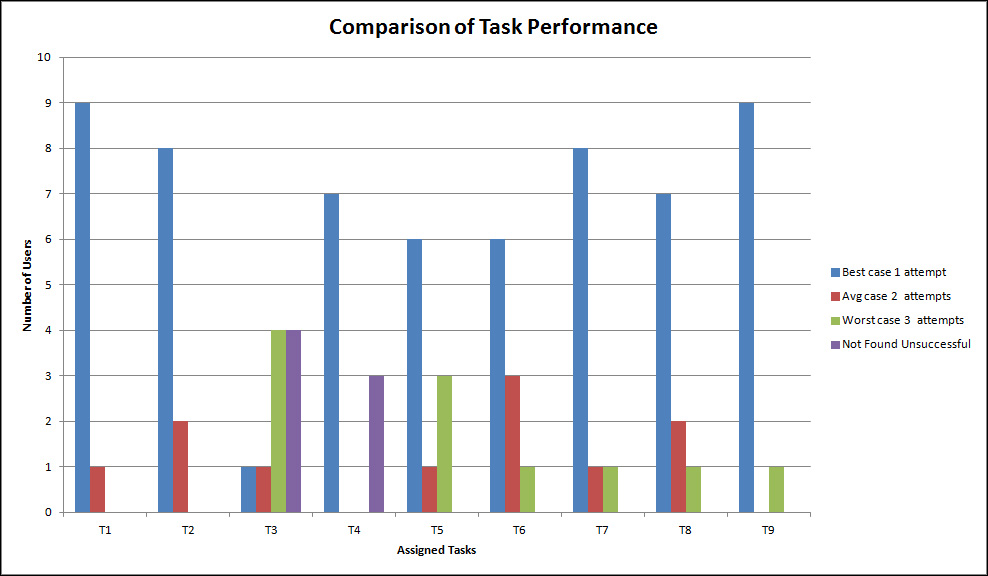
\includegraphics[width=5.5in,,height=3.5in]{ch5/Interview/EvaluationResult/ComparisonofTaskPerformance.jpg}
  \caption{Comparison of Tasks Performance.}
  \label{ComparisonofTasksPerformance}
\end{figure}

\subsection{Desktop Prototype Evaluation}
\label{subsec:QuestionnaireDesktop}
The study of the collected responses from the users through the questionnaire
has been presented in the tables bellow. In the
appendix[\ref{chap:UsabilityQuestionnaire}], questionnaire to measure usability
created in accordance with the USE questionnaire are provided
\cite{usabiltyUSE}. There was two part of questionnaire; firstly the general
information about the users and last part was for usability testing. The scale
of the questionnaire was based upon the Likert scale agreement or disagreement
within 7 point scale. The scale is as follows:

\begin{table}[h!t]
\centering
%\captionof{table}{Satisfaction} \label{tab:Satisfaction} 
 \begin{tabular}{| p{10cm} | p{2cm} |}
    \hline
      Likert Scale & Point  \\ \hline
      Strongly disagree & 1  \\ \hline
      Disagree & 2  \\ \hline
      More disagree than agree & 3  \\ \hline
      Neutral & 4  \\ \hline
      More agree than disagree & 5  \\ \hline
      Agree & 6  \\ \hline
      Strongly agree  & 7  \\ \hline   
    \end{tabular}
 \caption{Likert scale for Evaluation.}
\label{tab:Likertscale}
\end{table}

Ten users participated in the evaluation session. They have answered
14 usability questions which were labeled as Q1, Q2,\ldots and so on. Finally the
result was analyzed calculating Mean($\mu$) and Standard deviation($\sigma$).


Standard Deviation, $\sigma$ =  $\sqrt{\frac{1}{N}\sum_{i}^{N} (x_i - \mu^2)} $
where Mean, $\mu$ = $\frac{1}{N}\sum_{i}^{N} x_i$.

The reason of using Standard Deviation is to measure how spread feedback score
from Mean. Mean measures usability acceptance value; namely it belongs to below
neutral(scale 4)[not accepted] or upper regions from neutral(scale
4)[accepted][figure \ref{fig:EvaluationStatistics:Desktop}].


\subsubsection{Usefulness}
\label{subsub:Usefulness:Desktop}
In the first section of the questionnaire it was requested to the users for
providing their valuable feedback about the usefulness of smart cafeteria to
improve the system design.

\begin{table}[h!t]
\centering
%\captionof{table}{Usefulness} \label{tab:Usefulness} 
 \begin{tabular}{| p{6.2cm} | p{2cm} |p{4.3cm} | }
    \hline
    Questions & Mean ($\mu$) & Standard Deviation ($\sigma$) \\ \hline
    Q1. The smart cafeteria will help me to schedule my meal easily. & 4.9 & 1.663329993  \\ \hline
    Q2. This system will make my life more comfortable. & 4.3 & 1.766981104   \\   \hline
    Q3. This system will give me more control over the activities of my life. & 3.8 & 1.686548085 \\ \hline
    Q4. This system does everything I would expect it to do. & 4.3 & 1.636391694  \\   \hline
    \end{tabular}
 \caption{Usefulness[Desktop Prototype].}
\label{tab:Usefulness:Desktop}
\end{table}

From users' feedback result sheet [Appendix
\ref{sec:ResultforDesktopPrototype}], Usefulness of desktop prototype has been
calculated [Table \ref{tab:Usefulness:Desktop}]. The result sheet has shown that
``Smart Cafeteria'' system makes life easy at university and most of the users
agreed with usefulness of the new system. A significant number of users agreed
that by using this system they could find out their lunch menu easily. Half of
the user agreed that the system could make life comfortable and give more
control over activities of life; specially time at university.

\subsubsection{Ease of Use}
\label{subsub:EaseofUse:Desktop}
In second section of questionnaire, the feedback about ease of use of the ``Smart
Cafeteria'' was provided.

\begin{table}[h!t]
\centering
%\captionof{table}{Ease of Use} \label{tab:EaseofUse} 
 \begin{tabular}{| p{6.2cm} | p{2cm} |p{4.3cm} | }
    \hline
    Questions & Mean ($\mu$) & Standard Deviation ($\sigma$) \\ \hline
    Q5. The system is easy to use. & 4.9 & 1.33749351  \\ \hline
    Q6. The system requires fewest steps to accomplish what I want to do with it. & 5.1 & 1.370320319 \\ \hline
    Q7. I can use it without any written instruction. & 4.4 & 1.95505044 \\ \hline
    Q8. The system is user friendly. & 5.4 &  1.429840706 \\  \hline
    \end{tabular}
 \caption{Ease of Use [Desktop Prototype].}
\label{tab:EaseofUse:Desktop}
\end{table}

Table ``Ease of Use [Desktop Prototype]" [\ref{tab:EaseofUse:Desktop}] has been
generated from users' feedback result sheet for evaluating desktop prototype of
``Smart Cafeteria'' [Appendix \ref{sec:ResultforDesktopPrototype}]. The feedback
result has indicated that most users feel the software is easy to use and user
friendly but they have strong suggestion to include any written or visual
instruction of how to use the system.

\subsubsection{Ease of Learning}
\label{subsub:EaseofLearning:Desktop}
In the third section of questionnaire, users were asked to provide their opinion
about the system complexity of learnability.

\begin{table}[h!t]
\centering
%\captionof{table}{Ease of Learning} \label{tab:EaseofLearning} 
 \begin{tabular}{| p{6.2cm} | p{2cm} |p{4.3cm} | }
    \hline
    Questions & Mean ($\mu$) & Standard Deviation ($\sigma$) \\ \hline
    Q9. I learned to use it quickly. & 4.9 & 1.054092553 \\ \hline
    Q10. I easily remember how to use it. & 5.4 & 1.264911064 \\ \hline
    \end{tabular}
 \caption{Ease of Learning [Desktop Prototype].}
\label{tab:EaseofLearning:Desktop}
\end{table}

Table ``Ease of Learning [Desktop Prototype]" [\ref{tab:EaseofLearning:Desktop}] has
been calculated from users' feedback result sheet to evaluate desktop
prototype [Appendix \ref{sec:ResultforDesktopPrototype}]. In the feedback, more
than half of the users agreed that the desktop prototype is ease to learn.

\subsubsection{Satisfaction}
\label{subsub:Satisfaction:Desktop}
In the forth section of the questionnaire, users were asked to provide their
feedback about level of satisfaction after using the system.

\begin{table}[h!t]
\centering
%\captionof{table}{Satisfaction} \label{tab:Satisfaction} 
 \begin{tabular}{| p{6.2cm} | p{2cm} |p{4.3cm} | }
    \hline
    Questions & Mean ($\mu$) & Standard Deviation ($\sigma$) \\ \hline
    Q11. I am satisfied with it. & 4.9 & 1.888562063 \\ \hline
    Q12. It is fun to use. & 4.4 & 1.429840706 \\ \hline
    Q13. I feel I have to need it. & 4.9 & 1.286683938  \\ \hline
    Q14. I would recommend this to my friend. & 5.8 & 1.398411798 \\ \hline
    \end{tabular}
 \caption{Satisfaction [Desktop Prototype].}
\label{tab:Satisfaction:Desktop}
\end{table}

The table ``Satisfaction [Desktop Prototype]" [\ref{tab:Satisfaction:Desktop}]
has been deduced from users' feedback result sheet to evaluate desktop prototype
[Appendix \ref{sec:ResultforDesktopPrototype}]. The result sheet has shown that
more than half of the users were satisfied with the system and recommended the
system to their friends. Besides, to make the system more fun and enjoyable, it
needs more research to find out how we could make the system more fun and
attractable.

\subsubsection{Evaluation Statistics}
\label{subsub:EvaluationStatistics:Desktop}
The figure \ref{fig:EvaluationStatistics:Desktop} has shown that Q1, Q2 and Q4
feedback scores are more than neutral(scale 4) which deduces that Smart
cafeteria is usefull application in univesity. The feedback scores of questions
Q5, Q6, Q7 and Q8 are more than neutral(scale 4) which has proved that the
desktop prototype [\ref{subsec:prototypefordesktop}] of the application is easy
to use. The mean value of Q9, Q10 are more than neutral(scale 4) which ensured
that the desktop prototype [\ref{subsec:prototypefordesktop}] of the application
is easy to learn. The mean value of Q11, Q12, Q13 and Q14 are more than
neutral(scale 4) which make sure users' satisfaction when they use the system in
desktop's browser.

\begin{figure}[h!t]
    \centering
      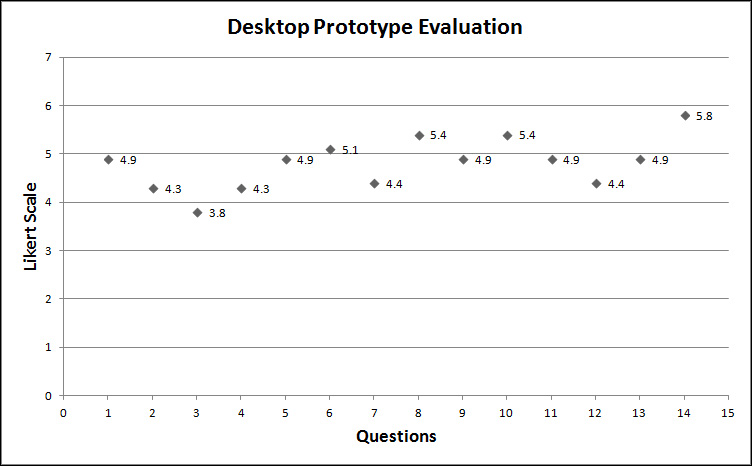
\includegraphics[width=5.5in,,height=3.5in]{ch5/Interview/EvaluationResult/UsabilityEvaluationGraphDesktop.jpg}
  \caption{Desktop Evaluation Statistics.}
  \label{fig:EvaluationStatistics:Desktop}
\end{figure}

\newpage

\subsection{Mobile Prototype Evaluation}
\label{subsec:QuestionnaireMobile}
Mobile prototype usability evaluation has followed similar procedure as desktop
prototype evaluation [\ref{subsec:QuestionnaireDesktop}]; same amount of
users(10) have participated and same questionnaire was provided. The same
techniques has been followed or analyzing the result
[\ref{subsub:EvaluationStatistics:Mobile}]. In the following section I have
analyzed the result of mobile prototype usability evaluation [Appendix
\ref{sec:ResultforMobilePrototype}].

\subsubsection{Usefulness}
\label{subsub:Usefulness:Mobile}
\begin{table}[h!t]
\centering
%\captionof{table}{Usefulness} \label{tab:Usefulness} 
 \begin{tabular}{| p{6.2cm} | p{2cm} |p{4.3cm} | }
    \hline
    Questions & Mean ($\mu$) & Standard Deviation ($\sigma$) \\ \hline
    Q1. The smart cafeteria will help me to schedule my meal easily. & 5.9 & 1.100504935 \\ \hline
    Q2. This system will make my life more comfortable. & 5.5 & 1.178511302  \\   \hline
    Q3. This system will give me more control over the activities of my life. & 4.6 & 1.577621275 \\ \hline
    Q4. This system does everything I would expect it to do. & 5.4 & 0.966091783  \\   \hline
    \end{tabular}
 \caption{Usefulness of Smart cafeteria.}
\label{tab:Usefulness:Mobile}
\end{table}

Table \ref{tab:Usefulness:Mobile} has concluded that ``Smart Cafeteria'' will be
more usefull; specially when it will be accessible through mobile. Above 70\%
users agreed to the usefullness of ``Smart Cafeteria'' mobile application [Appendix
\ref{sec:ResultforMobilePrototype}].

\subsubsection{Ease of Use}
\label{subsub:EaseofUse:Mobile}
\begin{table}[h!t]
\centering
%\captionof{table}{Ease of Use} \label{tab:EaseofUse} 
 \begin{tabular}{| p{6.2cm} | p{2cm} |p{4.3cm} | }
    \hline
    Questions & Mean ($\mu$) & Standard Deviation ($\sigma$) \\ \hline
    Q5. The system is easy to use. & 6.1 & 0.737864787  \\ \hline
    Q6. The system requires fewest steps to accomplish what I want to do with it. & 6 & 0.816496581 \\ \hline
    Q7. I can use it without any written instruction. & 5.8 & 1.135292424 \\ \hline
    Q8. The system is user friendly. & 5.6 &  0.966091783 \\  \hline
    \end{tabular}
 \caption{Ease of Use of Smart cafeteria.}
\label{tab:EaseofUse:Mobile}
\end{table}

Table \ref{tab:EaseofUse:Mobile} has drawn a conclusion that mobile ``Smart
Cafeteria'' is easy to use. Above 80\% of users agreed with the fact that it is
easy to use [Appendix \ref{sec:ResultforMobilePrototype}].

\subsubsection{Ease of Learning}
\label{subsub:EaseofLearning:Mobile}
\begin{table}[h!t]
\centering
%\captionof{table}{Ease of Learning} \label{tab:EaseofLearning} 
 \begin{tabular}{| p{6.2cm} | p{2cm} |p{4.3cm} | }
    \hline
    Questions & Mean ($\mu$) & Standard Deviation ($\sigma$) \\ \hline
    Q9. I learned to use it quickly. & 6 & 1.054092553 \\ \hline
    Q10. I easily remember how to use it. & 6.1 & 0.567646212 \\ \hline
    \end{tabular}
 \caption{Ease of Learning of Smart cafeteria.}
\label{tab:EaseofLearning:Mobile}
\end{table}
Table \ref{tab:EaseofLearning:Mobile} has concluded that users were agreed that
the mobile application is ease to learn.

\subsubsection{Satisfaction}
\label{subsub:Satisfaction:Mobile}
\begin{table}[h!t]
\centering
%\captionof{table}{Satisfaction} \label{tab:Satisfaction} 
 \begin{tabular}{| p{6.2cm} | p{2cm} |p{4.3cm} | }
    \hline
    Questions & Mean ($\mu$) & Standard Deviation ($\sigma$) \\ \hline
    Q11. I am satisfied with it. & 5.2 & 1.135292424 \\ \hline
    Q12. It is fun to use. & 4.6 & 1.429840706 \\ \hline
    Q13. I feel I have to need it. & 5.3 & 1.766981104  \\ \hline
    Q14. I would recommend this to my friend. & 5.8 & 1.475729575 \\ \hline
    \end{tabular}
 \caption{Satisfaction of Smart cafeteria.}
\label{tab:Satisfaction:Mobile}
\end{table}
The table \ref{tab:Satisfaction:Mobile} has deduced the average satisfactory
level which are more than neutral opinion of using ``Smart Cafeteria'' mobile
application.

\subsubsection{Evaluation Statistics}
\label{subsub:EvaluationStatistics:Mobile}
The figure \ref{fig:EvaluationStatistics:Mobile} has shown that Q1, Q2, Q3 and
Q4 feedback scores are more than scale 5 which deduces that ``Smart Cafeteria"
mobile application is usefull. The feedback scores of questions Q5, Q6, Q7 and
Q8 are more than scale 5 which has proved that the mobile
prototype[\ref{subsec:PrototypeforMobile}] of the application is easy to use.
The mean value of Q9, Q10 are more than scale 5 which ensured that the mobile
prototype[\ref{subsec:PrototypeforMobile}] is easy to learn. The mean value of
Q11, Q12, Q13 and Q14 are more than neutral(scale 4) which make sure users'
satisfaction when they use ``Smart Cafeteria" in mobile.

\begin{figure}[h!t]
    \centering
      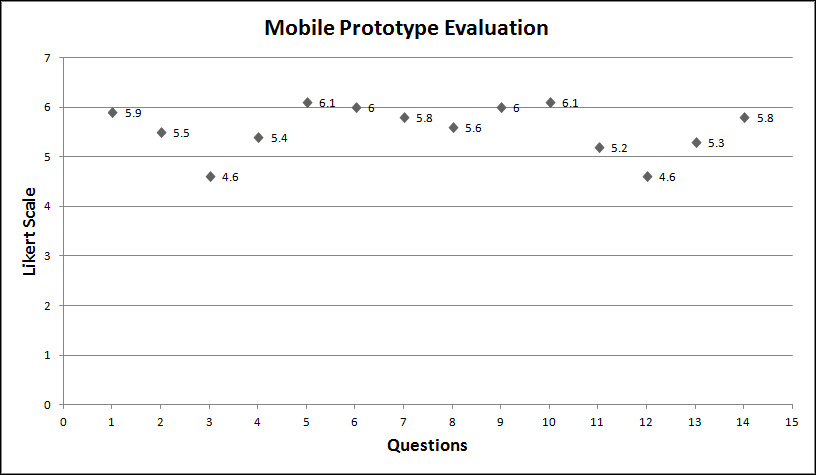
\includegraphics[width=5.5in,,height=3.5in]{ch5/Interview/EvaluationResult/UsabilityEvaluationGraphMobile.jpg}
  \caption{Mobile Evaluation Statistics.}
  \label{fig:EvaluationStatistics:Mobile}
\end{figure}


\section{Suggestions for Improvement}
The last three questions were open question to users about their suggestions,
comments about the system and which part they like most. Finally analysis of the
qualitative data we have found the following facts.

\begin{itemize}
  \item Users mostly liked parts in the system are they could know about the
  updates of food menu everyday, time schedule of cafeteria, serve menu on time
  means no queue time, dieting suggestion e.g. suggest food menu, dieting report
  e.g. calorie consumptions per month. Users also like adaptability of the
  system which is responsible for generating automatic menu suggestions and create
  customized menu functionality. Users like social collaboration activities such
  as food menu's pictures, url and real time odrer activity with friends.
  \item This part is open suggestions and comments from users. They want to see the
  following things:
  \begin{itemize}
    \item Help instruction should be provided using short video.
    \item Advanced customized food menu booking system and that should be
    clearly define with drag and drop action.
    \item Provide waiting time notification after booking the lunch. Time of
    delivery can be included with time flexibilities (In case of emergency user
    can postponed the delivery time).
    \item Inviting friends from other social media or let them know about this
    application.
    \item Brief summary of monthly calorie consumption in front page.
    \item Want to know which cafeteria is less crowded at lunch time.
    \item Should indicate which food menus are Halal(for Muslim people).
    \item Should clarify that different prices for different stakeholder;
    e.g.  Students will pay at discount rate.
    \item Should have users flexibility in cancel order or delay order option.
   \end{itemize}
\end{itemize}
Since this was the first time evaluation and user study, UI navigation and
control should be improved such that user will not face difficulties and could
understand what's going on in the system. It should include all the new
requirements of the system and conducted more survey and evaluation.
